	
\chapter{Setting itlx3304}


\begin{itemize}
 \item Apache configuration
 \subitem wwwitrt.conf
 \subitem dav\_svn.conf
 \subitem jk.conf
 \subitem shibboleth.conf
 \item LDAP configuration
 \item Jenkins configuration
 \item SVN configuration
 \item Trackplus configuration
 \item MySql configuration
 \item PWM configuration
\end{itemize}

\section{Trackplus Configuration}
To integrate Jenkins and other web applications in trackplus, we need to
download portal$5.0$ from the trackplus website. This plugin has to be
configured and urls of the webapplications needs to be written in the
configuration file inside the portal$5.0$ directory.
The plugin to be downloaded from the trackplus website has the extension .tpx.
 
\section{MySql configuration}
MySql is a database and needs to be configured for trackplus. First of all a
database is created, but for that one needs to know the root password of MySql.
The root password is kept under the folder called /root in the server.
mysql -uroot -ptissi
mysql -utrackp -ptissi
mysql -uroot -p (password in the /root folder)


\chapter{Removing legacy code from SVN}
\section{Deleting and
moving old SVN Repositories in itlx3301}As of August, $22015$, there were seven
SVN repositories excluding lab team repositories\\\\
\begin{figure}[H]
\begin{center}
		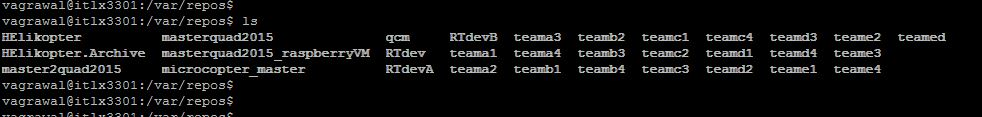
\includegraphics[width=1.0\textwidth]{images/svn_repos_before.jpg} 
		\caption{Repos before changes}
	\label{fig:SVNBefore}
\end{center}
\end{figure}

\begin{enumerate}
  \item HElikopter
  \item HElikopter.Archive
  \item microcopter\_master
  \item masterquad$2015$
  \item masterquad$2015$\_raspberryVM
  \item master$2$quad$2015$
  \item DOSEK
\end{enumerate}

\section{Moving the repositories}
\begin{itemize} 
  \item
  \textbf{HElikopter}
  \url{svn+ssh://vagrawal@itlx3301.hs-esslingen.de/var/repos/HElikopter/trunk} This is the HElikopter source code on the code warrior and is maintaned by Hr.
  Trybek. The underlying microcontroller is the dragon board running the
  Freescale microcontroller. The project has the milestone REL$210$ as of
  $01.10.2014$.
  The repositories HElikopter is merged into git repoitories kept at
  \url{https://atreus.informatik.uni-tuebingen.de/agrawal/helikopter-software}.
  However the svn repository still exists since Hr Trybek works on the
  repository.
  
  \item
  \textbf{HElikopter.Archive}
  \url{svn+ssh://vagrawal@itlx3301.hs-esslingen.de/var/repos/HElikopter.Archive} This is a legacy project and has two tags REL$100$ from
  $24.04.2012$ and REL$200$ from $25.03.2013$.
  The SVN repository HElikopter.archive is moved to the
  Trash folder in /var/repos/. 
  The repositories HElikopteris merged into git repository kept at
  \url{https://atreus.informatik.uni-tuebingen.de/agrawal/helikopter-software},
  \item
  \textbf{microcopter\_master}
  \url{svn+ssh://vagrawal@itlx3301.hs-esslingen.de/var/repos/microcopter_master}
  The project also consists of the development of the HElikopter and consists of
  the matlab projects as well as the codewarrior projects. Last development in
  the project was in the year $2011$. This SVN repository has been moved to
  Trash under /var/repos and the contents has been merged in 
  \url{https://atreus.informatik.uni-tuebingen.de/agrawal/helikopter-simulation}
  and
  \url{https://atreus.informatik.uni-tuebingen.de/agrawal/helikopter-scratch}.
  \item
  \textbf{master2quad2015}
  \url{svn+ssh://vagrawal@itlx3301.hs-esslingen.de/var/repos/master2quad2015}
  This is a masters student $2015$ matlab project to make a matlab model of
  the HElikopter. This repository is deleted and the contents has been merged
  in the GIT repo \url{https://atreus.informatik.uni-tuebingen.de/agrawal/helikopter-simulation}
  \item
  \textbf{masterquad$2015$ and masterquad$2015$\_raspberryVM}
  \url{svn+ssh://vagrawal@itlx3301.hs-esslingen.de/var/repos/masterquad2015}
  This is a masters student $2015$ respberry project to make a raspberry based
  development of the HElikopter. The project consists of the ubuntu virtual
  machine which is a development environment and the source files consisting of
  the application and low lever drivers written for the raspberry.\\
  The repository masterquad$2015$ is moved to Trash under /var/repos and the
  content has been moved to two GIT Repositories.
  \url{https://atreus.informatik.uni-tuebingen.de/agrawal/helikopter-vm}
  and
  \url{https://atreus.informatik.uni-tuebingen.de/agrawal/helikopter-raspberry}.
  \item
  \textbf{LAB Team Repositores}
  The lab team project repositories are moved under the folder /var/repos/LABOR.
  \item
  \textbf{DOSEK}
  The DOSEK repositories are moved under the folder /var/repos/DOSEK.
  \end{itemize}
  
\section{SVN Repositories after changes}Now there are only two SVN
repositories excluding the lab team repositories\\
\begin{figure}[H]
\begin{center}
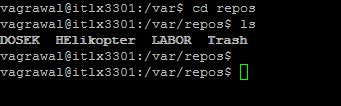
\includegraphics[width=1.0\textwidth]{images/svn_repos_after.jpg} 
\caption{Repos after changes}
\label{fig:SVNAfter}
\end{center}
\end{figure}
\begin{enumerate}
  \item HElikopter
  \item DOSEK
\end{enumerate}



\section{Exercises}
Team of Controller, Actuator and UI 
The students would study about the communication buses such as I2C, SPI, UART,
CAN.

\section{Slides}
\textbf{Estimation} : The process of inferring a value of a quantity of interest
from indirect, inaccurate and uncertain observations is called estimation.



\begin{figure}[H]
\begin{center}
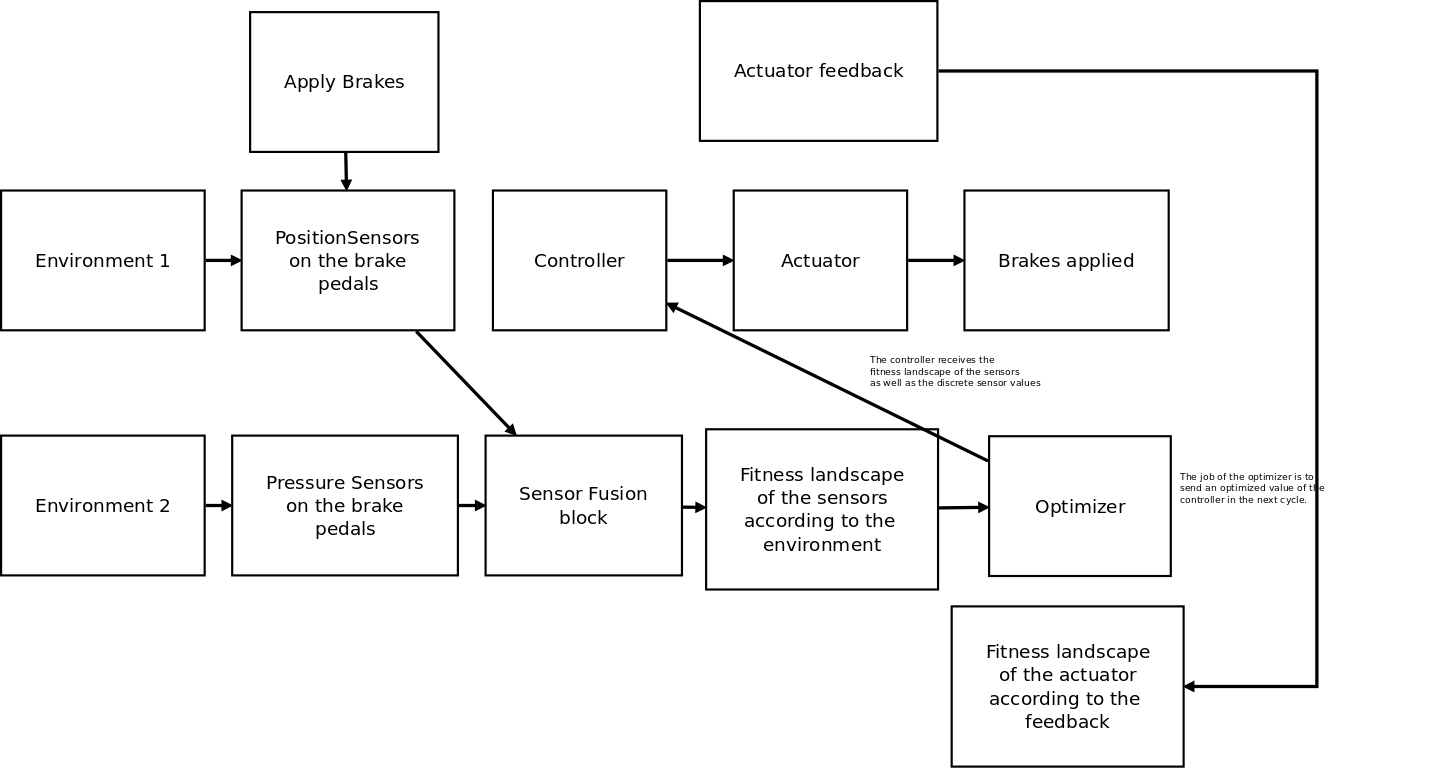
\includegraphics[width=1.0\textwidth]{images/second.png}
\caption{Overview}
\label{fig:Overview}
\end{center}
\end{figure}
